\chapter*{Dodatak: Prikaz aktivnosti grupe}
		\addcontentsline{toc}{chapter}{Dodatak: Prikaz aktivnosti grupe}
		
		\section*{Dnevnik sastajanja}
		
		
		\begin{packed_enum}
			\item  sastanak
			
			\item[] \begin{packed_item}
				\item Datum: 2. listopada 2020.
				\item Prisustvovali: I.Bokšić, I.Jakas, M.Lipovac, M.Oreč, J.Roček, R.Đaković, D.Ćurić
				\item Teme sastanka:
				\begin{packed_item}
					\item  upoznavanje tima
					\item  razgovor o projektu i trenutnim tehnološkim znanjima članova
				\end{packed_item}
			\end{packed_item}
			
				\item  sastanak
			\item[] \begin{packed_item}
				\item Datum: 8. listopada 2020.
				\item Prisustvovali: I.Bokšić, I.Jakas, M.Lipovac, M.Oreč, J.Roček, R.Đaković, D.Ćurić
				\item Teme sastanka:
				\begin{packed_item}
					\item  razgovor s asistenticom i demostratorom
					\item analiza projekta
					\item razješavanje prvih nedoumica oko zadatka 
				\end{packed_item}
			\end{packed_item}
		
			\item  sastanak
			\item[] \begin{packed_item}
				\item Datum: 10. listopada 2020.
				\item Prisustvovali: I.Bokšić, I.Jakas, M.Lipovac, M.Oreč, J.Roček, R.Đaković, D.Ćurić
				\item Teme sastanka:
				\begin{packed_item}
					\item  razgovor o tehnologijama koje ćemo koristiti i njihova instalacija
					\item  okvirna podjela rada
				\end{packed_item}
			\end{packed_item}
			
			
				\item  sastanak
			\item[] \begin{packed_item}
				\item Datum: 14. listopada 2020.
				\item Prisustvovali: I.Bokšić, I.Jakas, M.Lipovac, M.Oreč, J.Roček, R.Đaković, D.Ćurić
				\item Teme sastanka:
				\begin{packed_item}
					\item definiranje funkcionalnih zahtjeva 
					\item kreiranje use case dijagrama
				\end{packed_item}
			\end{packed_item}
			%
				\item  sastanak
			\item[] \begin{packed_item}
				\item Datum: 16. listopada 2020.
				\item Prisustvovali: I.Bokšić, M.Lipovac, M.Oreč, J.Roček, R.Đaković, D.Ćurić
				\item Teme sastanka:
				\begin{packed_item}
					\item konačno definiranje use case dijagrama
					\item nova podjela zadataka
				\end{packed_item}
			\end{packed_item}
			%
	
		\item  sastanak
		\item[] \begin{packed_item}
			\item Datum:  26. listopada 2020.
			\item Prisustvovali: D.Ćurić
			\item Teme sastanka:
			\begin{packed_item}
				\item razgovor s asistenticom i demostratorom
				\item rasprava o sekvencijskim dijagramima
			\end{packed_item}
		\end{packed_item}
		%

			\item  sastanak
		\item[] \begin{packed_item}
			\item Datum: 3. studenog 2020.
			\item Prisustvovali: I.Bokšić, M.Lipovac, R.Đaković, D.Ćurić
			\item Teme sastanka:
			\begin{packed_item}
				\item raspodijela posla na dokumentaciji 
				\item prezentiranje login i  sign in stranice  
			\end{packed_item}
		\end{packed_item}
		%
		
			\item  sastanak
		\item[] \begin{packed_item}
			\item Datum: 3. studenog 2020.
			\item Prisustvovali: J.Roček
			\item Teme sastanka:
			\begin{packed_item}
				\item razgovor s demonstratorom  
				\item rasprava oko implementacije JWT-a 
			\end{packed_item}
		\end{packed_item}
		%
		
			\item  sastanak
		\item[] \begin{packed_item}
			\item Datum: 5. studenog 2020.
			\item Prisustvovali: I.Bokšić, I.Jakas, M.Lipovac, M.Oreč, J.Roček, R.Đaković, D.Ćurić
			\item Teme sastanka:
			\begin{packed_item}
				\item razgovor s asistenticom i demostratorom
				\item komentiranje dijagrama baze podataka
				\item sugestija oko izrade dijagrama razreda
			\end{packed_item}
		\end{packed_item}
		%
		
		  \item  sastanak
		\item[] \begin{packed_item}
			\item Datum: 10. prosinca 2020.
			\item Prisustvovali: J.Roček, D.Ćurić, M.Oreč, M.Lipovac
			\item Teme sastanka:
			\begin{packed_item}
				\item dogovor oko implementacijskih detalja vezanih
				     uz backend
			\end{packed_item}
		\end{packed_item}
		%
		
			\item  sastanak
		\item[] \begin{packed_item}
			\item Datum: 15. prosinac 2020.
			\item Prisustvovali:J.Roček, D.Ćurić 
			\item Teme sastanka:
			\begin{packed_item}
				\item pregled napravljenih dijelova backend
				\item definiranje novih zadataka za backend
				
			\end{packed_item}
		\end{packed_item}
		%
		
			\item  sastanak
		\item[] \begin{packed_item}
			\item Datum: 17. prosinca 2020.
			\item Prisustvovali: J.Roček, M.Oreč, M.Lipovac 
			\item Teme sastanka:
			\begin{packed_item}
				\item pregled napravljenih dijelova backend
			    \item definiranje novih zadataka za backend
			\end{packed_item}
		\end{packed_item}
		%
		
			\item  sastanak
		\item[] \begin{packed_item}
			\item Datum: 22. prosinca 2020.
			\item Prisustvovali: J.Roček, D.Ćurić 
			\item Teme sastanka:
			\begin{packed_item}
				\item pregled napravljenih dijelova backend
			    \item modificiranje postojećih metoda 
			    \item definiranje novih zadataka za backend
			\end{packed_item}
		\end{packed_item}
		%
		
		    \item  sastanak
		\item[] \begin{packed_item}
			\item Datum: 23. prosinca 2020.
			\item Prisustvovali: J.Roček, I.Jakas, R.Đaković, I.Bokšić
			\item Teme sastanka:
			\begin{packed_item}
				\item pregled napravljenih dijelova backend
			    \item definiranje zadataka za frontend
			\end{packed_item}
		\end{packed_item}
		%
		
		\item  sastanak
		\item[] \begin{packed_item}
			\item Datum: 27. prosinca 2020.
			\item Prisustvovali: I.Jakas, R.Đaković, I.Bokšić
			\item Teme sastanka:
			\begin{packed_item}
				\item pregled rada na frontu
				\item definiranje novih zadataka na frontu
			\end{packed_item}
		\end{packed_item}
		%
		
			\item  sastanak
		\item[] \begin{packed_item}
			\item Datum: 3. siječnja 2021.
			\item Prisustvovali: J.Roček, M.Oreč, M.LIpovac
			\item Teme sastanka:
			\begin{packed_item}
				\item dogovor oko pisanja JUnit testova
			    \item dogovor oko same implementacije JUnit testova
			\end{packed_item}
		\end{packed_item}
		%
		
		\item  sastanak
		\item[] \begin{packed_item}
			\item Datum: 4. siječnja 2020.
			\item Prisustvovali: I.Jakas, R.Đaković, I.Bokšić, J.Roček
			\item Teme sastanka:
			\begin{packed_item}
				\item pregled fronta 
				\item novo definiranje zadataka
			\end{packed_item}
		\end{packed_item}
		%
		
		\item  sastanak
		\item[] \begin{packed_item}
			\item Datum: 7. siječnja 2020.
			\item Prisustvovali: I.Jakas, R.Đaković, I.Bokšić, J.Roček, M.Lipovac, M.Oreč, D.Ćurić
			\item Teme sastanka:
			\begin{packed_item}
				\item demonstriranje alfa verzije asistentici 
				\item popravci funkcionalnosti
			\end{packed_item}
		\end{packed_item}
		%
		
		\item  sastanak
		\item[] \begin{packed_item}
			\item Datum: 13. siječnja 2021.
			\item Prisustvovali: J.Roček, R.Đaković, I. Bokšić
			\item Teme sastanka:
			\begin{packed_item}
				\item konačni pregled aplikacije i popravci
				\item rasprava oko dokumentacije
			\end{packed_item}
		\end{packed_item}
		%
		
	\end{packed_enum}

		
		
		\eject
		\section*{Tablica aktivnosti}
		
		%	\textbf{\textit{Kontinuirano osvježavanje}}\\
			
		%	 \textit{Napomena: Doprinose u aktivnostima treba navesti u satima po članovima grupe po aktivnosti.}
					
						
			
			\begin{longtabu} to \textwidth {|X[7, l]|X[1, c]|X[1, c]|X[1, c]|X[1, c]|X[1, c]|X[1, c]|X[1, c]|}
								
				\cline{2-8} \multicolumn{1}{c|}{\textbf{}} &     
				\multicolumn{1}{c|}{\rotatebox{90}{\textbf{Iva Bokšić }}} & \multicolumn{1}{c|}{\rotatebox{90}{\textbf{Jan Roček }}} &	\multicolumn{1}{c|}{\rotatebox{90}{\textbf{Ivan Jakas }}} &	\multicolumn{1}{c|}{\rotatebox{90}{\textbf{Robert Đaković }}} &
				\multicolumn{1}{c|}{\rotatebox{90}{\textbf{Matea Lipovac}}} &
				\multicolumn{1}{c|}{\rotatebox{90}{\textbf{Dominik Ćurić }}} &	\multicolumn{1}{c|}{\rotatebox{90}{\textbf{Marija Oreč }}} \\ \hline 
				\endfirsthead
				
			
				\cline{2-8} \multicolumn{1}{c|}{\textbf{}} &     
				\multicolumn{1}{c|}{\rotatebox{90}{\textbf{Iva Bokšić }}} & \multicolumn{1}{c|}{\rotatebox{90}{\textbf{Jan Roček }}} &	\multicolumn{1}{c|}{\rotatebox{90}{\textbf{Ivan Jakas }}} &	\multicolumn{1}{c|}{\rotatebox{90}{\textbf{Robert Đaković }}} &
				\multicolumn{1}{c|}{\rotatebox{90}{\textbf{Matea Lipovac}}} &
				\multicolumn{1}{c|}{\rotatebox{90}{\textbf{Dominik Ćurić }}} &	\multicolumn{1}{c|}{\rotatebox{90}{\textbf{Marija Oreč }}} \\ \hline 
				\endhead
				
				
				\endfoot
							
				 
				\endlastfoot
				
				Upravljanje projektom 		&2  &3  &2  &1  &  &  & \\ \hline
				Opis projektnog zadatka 	&  &  &  &  &  &  &5 \\ \hline
				
				Funkcionalni zahtjevi       &1  &1  &1  &1  &1  &1  &1  \\ \hline
				Opis pojedinih obrazaca 	&4  &   &  &  &6  &  &  \\ \hline
				Dijagram obrazaca 			&2  &3  &  &1  &  &1  &2  \\ \hline
				Sekvencijski dijagrami 		&  &  &2  &2  &  &5  &  \\ \hline
				Opis ostalih zahtjeva 		&  &  &  &  &  &  &1  \\ \hline

				Arhitektura i dizajn sustava	 &4  &2  &  &  &  &  &  \\ \hline
				Baza podataka				&2  &5  &  &  &1  &1  &   \\ \hline
				Dijagram razreda 			&1  &  &  &  &2  &  &3   \\ \hline
				Dijagram stanja				&  &  &  &  &  &7  &  \\ \hline
				Dijagram aktivnosti 		&  &  &  &  &  &4  &  \\ \hline
				Dijagram komponenti			&  &  &  &  &  &4  &  \\ \hline
				Korištene tehnologije i alati 		&  &  &  &  &  &1  &  \\ \hline
				Ispitivanje programskog rješenja 	&  &1  &  &  &10  &  &10  \\ \hline
				Dijagram razmještaja			&  &  &  &  &  &1  &  \\ \hline
				Upute za puštanje u pogon 		&1  &1  &  &  &  &  &  \\ \hline 
				Dnevnik sastajanja 			&1  &  &  &  &  &1  &  \\ \hline
				Zaključak i budući rad 		&  &  &  &  &2  &  &2  \\  \hline
				Popis literature 			&1  &  &  &  &  &  &  \\  \hline
				Izrada login stranice			&1  &  &3  &1  &  &  &  \\ \hline 
				Izrada baze podataka 		 			&1  &2  &  &  &  &  & \\ \hline 
				Integriranje fronta i backa 	&  &15  &  &  &  &  &  \\ \hline
				Backend							&  &100  &  &  &20  &20  &20  \\  \hline
				Front							&50  &10  &70  &60  &  &  &  \\  \hline
				 							
				
				
			\end{longtabu}
				
			
			\eject
			\section*{Dijagrami pregleda promjena}
			
		
			
		%	\textit{Prenijeti dijagram pregleda promjena nad datotekama projekta. Potrebno je na kraju projekta generirane grafove s gitlaba prenijeti u ovo poglavlje dokumentacije. Dijagrami za vlastiti projekt se mogu preuzeti s gitlab.com stranice, u izborniku Repository, pritiskom na stavku Contributors.}
		
		\begin{figure}[H]
			\begin{center}
				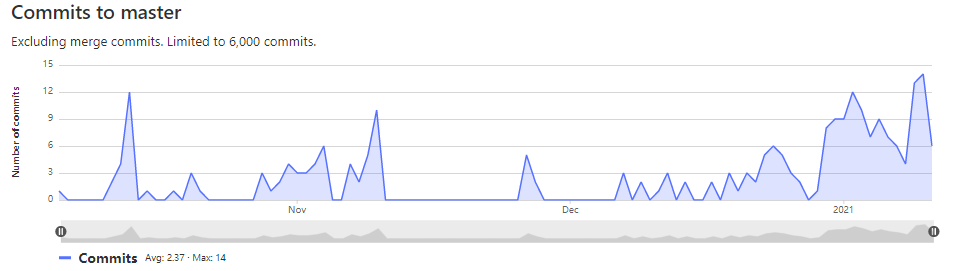
\includegraphics[width=15cm]{slike/master.png}
			\end{center}
			\caption{Dijagram pregleda promjena na grani master}
			\label{fig:master}
		\end{figure}
		
		\begin{figure}[H]
			\begin{center}
				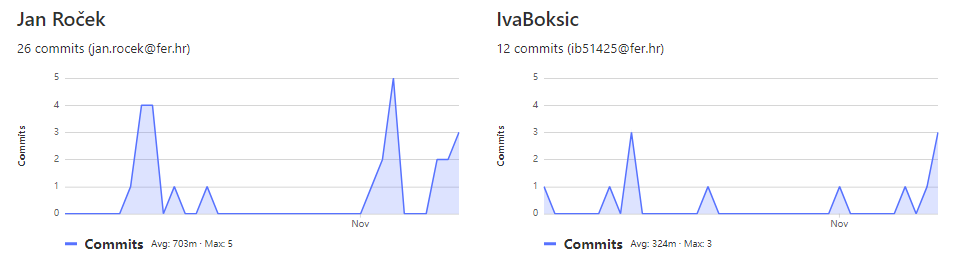
\includegraphics[width=15cm]{slike/master1.PNG}
				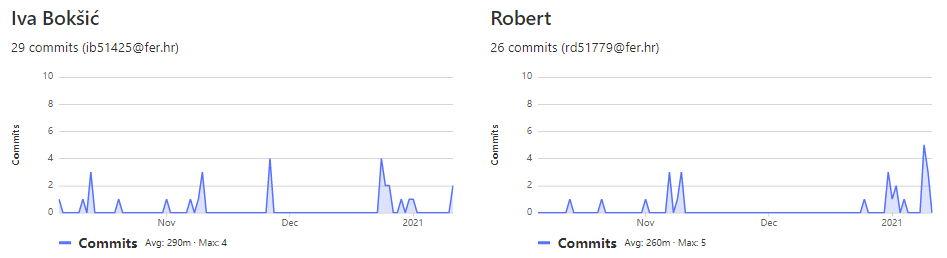
\includegraphics[width=15cm]{slike/master2.PNG}
				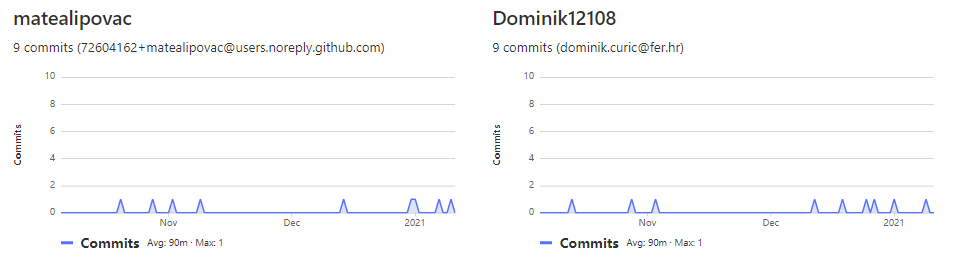
\includegraphics[width=15cm]{slike/master3.PNG}
				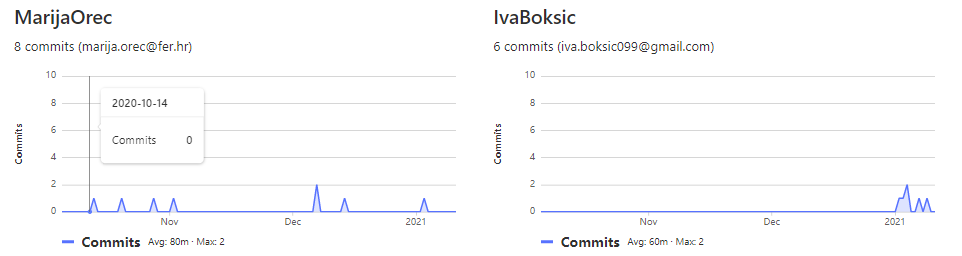
\includegraphics[width=15cm]{slike/master4.PNG}
				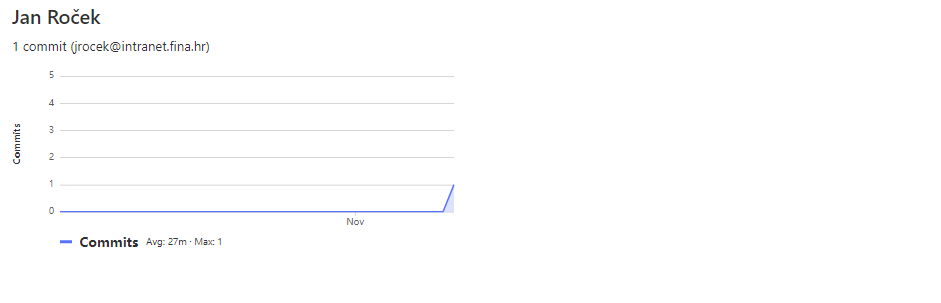
\includegraphics[width=15cm]{slike/master5.PNG}
			\end{center}
			\label{fig:dijapre}
		\end{figure}
	
	